% Project paper. Every symbol is defined where it first appears and in Table I.
% Numbers come from docs/handoff/phase3.md, results_phase3_ppo/README.md and results_phase4/.
\documentclass[conference]{IEEEtran}

\usepackage{amsmath,amssymb}
\usepackage{booktabs}
\usepackage{graphicx}
\usepackage{xcolor}
\usepackage{cite}
\usepackage{url}
\usepackage{tikz}
\usetikzlibrary{arrows.meta,positioning,calc}

\newcommand{\todo}[1]{\textcolor{red}{[TODO: #1]}}

\begin{document}

\title{Promise-Based Wake Scheduling for\\UAV Data Collection}

\author{\IEEEauthorblockN{Nihar Sagar G, Prakruthi K S, Shreya S Bhat, Balasani Thiaana}
\IEEEauthorblockA{Indian Institute of Technology Dharwad, Dharwad, India\\
\{ee23bt023, cs23bt062, cs23bt070, cs24bt031\}@iitdh.ac.in}}

\maketitle

\begin{abstract}
A UAV can collect the data of a wireless sensor network that has no base station by flying to
each cluster head (CH), but only if the CH has its radio on when the UAV arrives. This paper
studies how the visiting order of the UAV and the wake-up times of the CHs should be chosen
together. We propose a promise-then-honour wake rule, in which the UAV promises each CH its
return time and the CH listens only in a window around it, widened by the UAV's measured
lateness, and we implement the complete system in ns-3 with simulated Wi-Fi links, radio
energy, backup CHs and retry windows. On top of this rule, a PPO agent chooses the next cluster
by scoring every cluster from the UAV's own beliefs. On ten unseen networks, the agent delivers
97.3\% of the data, which is not significantly different from the shortest tour (97.2\%),
against 90.7\% for the best heuristic and 71.8\% for a tabular Q-learning baseline adapted from
prior work, and it keeps 3.6 times as many meetings as the best heuristic. Trained only on
100-sensor networks, it stays within 0.2 pp of the tour on hotspot networks with up to 2000
sensors and 20 clusters, where the heuristics lose up to 42 pp. In cases built to favour leaving
the tour, with small buffers and with sudden traffic bursts, a trained agent either follows the
tour or does worse. Our results show that once every CH sleeps until a promised time, the
shortest tour is already close to the best visiting order, and that the value of learning lies
in keeping promises reliably on networks of any size.
\end{abstract}

\begin{IEEEkeywords}
Wireless sensor networks, UAV data collection, wake scheduling, reinforcement learning, PPO,
ns-3.
\end{IEEEkeywords}

% ---------------------------------------------------------------------------------------------
\section{Introduction}

Sensor networks for environmental monitoring, farming or disaster areas are often deployed
where there is no cellular coverage and no fixed base station. The sensors are grouped into
clusters, and in each cluster one cluster head (CH) collects the readings of its members. A UAV
then flies from cluster to cluster and uploads each CH's buffer over Wi-Fi. This removes the
need for multi-hop relaying, but a CH can only upload while its Wi-Fi radio is on, and a CH that
listens all the time spends most of its energy waiting.

Two decisions therefore have to be made together: which cluster the UAV visits next, and when
each CH turns its radio on. Learning-based UAV routing
\cite{bayerlein2018trajectory,zhu2021uav,wang2022learning} usually assumes that the ground nodes
are always ready, and joint path and wake-up planning \cite{zhan2018energy} is solved offline for
a UAV that is never late. In practice the arrival time of the UAV varies, a sleeping CH cannot
be told about a change of plan, and a missed meeting may mean either a late UAV or a failed CH.
In our experiments, heuristics that plan from the UAV's beliefs keep only 19--25\% of their
meetings, and their CHs use 2.5 times the energy of a shortest tour. It is therefore unclear
which visiting order works when the CHs sleep, whether a learned policy can do better than a
fixed tour, and how such a policy behaves on networks it was not trained on.

In this paper, we study the problem from the side of the wake-up rule. Our results are
consistent with one account: \emph{once every CH sleeps until a time the UAV has promised it,
the shortest tour is already close to the best visiting order}. The account fits what a learned
policy does. A PPO agent that is free to choose any cluster ends up matching the tour, on the
networks it was trained on and on networks up to twenty times larger, and it beats every
heuristic by keeping its promises. The account also fits what fails. Every policy that leaves
the tour to chase data, whether a heuristic, a Q-learning baseline or a PPO agent that explores
more, makes the UAV late at the clusters it skips and loses both meetings and data. To test the
account directly, we build the two cases in which the tour should be easiest to beat, small
buffers and sudden traffic bursts, and train PPO on them.

\textbf{Problem statement.} A UAV collects data from $K$ clusters during a mission of fixed
length. It only knows what each CH reported at its last visit, and each CH sleeps outside a
window it was told in advance. We ask which visiting order maximises the data delivered while
keeping the meetings and the CH energy, whether a policy learned with PPO can improve on the
shortest tour, and whether such a policy transfers to larger and denser networks.

\textbf{Key contributions.} The main contributions of this paper are as follows.
\begin{itemize}
  \item \textbf{A promise-then-honour wake rule and its implementation.} At every visit the UAV
  promises the CH a return time, and the CH listens only in a window around it whose late side
  is set from the UAV's own lateness record (Section~\ref{sec:system}). All routing policies use
  the same rule, so they differ only in the order of visits. We implement the complete system
  in ns-3, with simulated Wi-Fi links and radio energy, backup CHs, retry windows and a
  start-up lap.
  \item \textbf{A PPO agent that matches the tour and beats every other policy.} The agent
  scores every cluster from its own beliefs with one shared network (Section~\ref{sec:method}).
  On ten unseen networks its PDR of 0.973 is not significantly different from the tour (0.972),
  and it beats the best heuristic (0.907) and a tabular Q-learning baseline adapted from
  Bouhamed et al.\ \cite{bouhamed2020uav} (0.718). We also report the training choices without
  which PPO kept only 59\% of its meetings.
  \item \textbf{Transfer to larger networks.} Trained only on 100-sensor networks, the agent stays
  within 0.2 pp of the tour on hotspot networks with up to 2000 sensors and 20 clusters, where
  the heuristics lose up to 42 pp and Q-learning drops to 0.27--0.55 (Section~\ref{sec:scale}).
  \item \textbf{A test of whether the tour can be beaten.} With small buffers and with event
  bursts, in which one cluster suddenly produces 20 times more data, a trained agent either
  follows the tour exactly or does worse (Section~\ref{sec:beat}).
\end{itemize}

The rest of the paper is organised as follows. Section~\ref{sec:related} reviews related work,
and Section~\ref{sec:system} describes the system model and the wake rule.
Section~\ref{sec:method} presents the PPO agent, Section~\ref{sec:setup} the experimental setup,
and Section~\ref{sec:results} the results. Section~\ref{sec:discussion} discusses them, and
Section~\ref{sec:conclusion} concludes.

% ---------------------------------------------------------------------------------------------
\section{Related Work}\label{sec:related}

\textbf{Clustering and sleep schedules.} LEACH \cite{heinzelman2002leach} rotates the CH role
so that no node runs out of energy first. S-MAC \cite{ye2002smac} puts nodes to sleep on a fixed
schedule to reduce idle listening, and Gupta and Younis \cite{gupta2003fault} add backup CHs. All
three assume a fixed sink that is always reachable.

\textbf{Mobile collectors and UAV paths.} Somasundara et al.\ \cite{somasundara2004mobile}
schedule a mobile collector against sensor deadlines with simple rules. Zhan et al.\
\cite{zhan2018energy} plan the UAV path and the sensor wake-up times together, but offline.
Zeng et al.\ \cite{zeng2019rotary} model the flight energy of a rotary-wing UAV, and Samir et
al.\ \cite{samir2020trajectory} plan paths for devices with deadlines. These methods assume that
the conditions are known in advance, so a single delay breaks the plan.

\textbf{Learning-based UAV data collection.} Bayerlein et al.\ \cite{bayerlein2018trajectory},
Zhu et al.\ \cite{zhu2021uav} and Wang et al.\ \cite{wang2022learning} plan UAV paths with
reinforcement learning, but treat the ground nodes as always ready. Bouhamed et al.\
\cite{bouhamed2020uav} choose the UAV's next sensor with tabular Q-learning over a small state
(location, time slot and battery), which we adapt as a learning baseline. Attention-based
policies for routing problems \cite{kool2019attention} inspired the network with which we score
clusters. In contrast to these methods, our agent plans from the UAV's estimates instead of
the true state, its reward includes the CH listening energy and missed meetings, and CH
failures are kept separate from UAV delays in a packet-level simulator.

% ---------------------------------------------------------------------------------------------
\section{System Model}\label{sec:system}

\begin{figure*}[t]
\centering
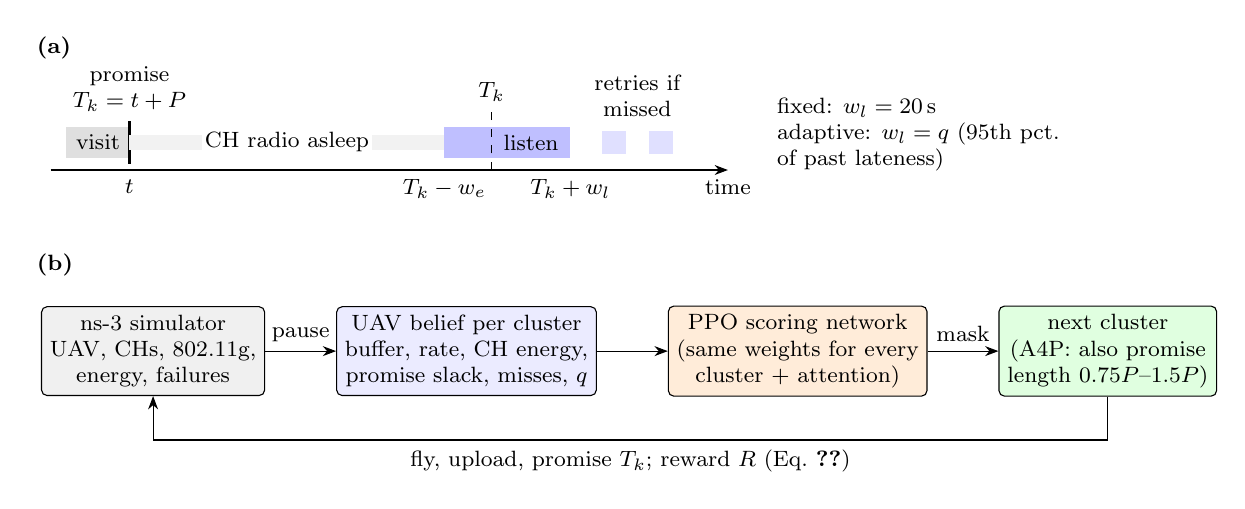
\begin{tikzpicture}[font=\footnotesize, >=Stealth,
  box/.style={draw, rounded corners=2pt, align=center, minimum height=8mm, inner sep=3pt}]
% (a) timeline of one promise
\node[anchor=west] at (-0.3,1.55) {\textbf{(a)}};
\draw[->] (0,0) -- (8.6,0) node[below] {time};
\fill[gray!25] (0.2,0.15) rectangle (1.0,0.55);
\node at (0.6,0.35) {visit};
\draw[very thick] (1.0,0.08) -- (1.0,0.62);
\node[above, align=center] at (1.0,0.62) {promise\\$T_k = t + P$};
\node[below] at (1.0,0) {$t$};
\fill[gray!10] (1.0,0.25) rectangle (5.0,0.45);
\node at (3.0,0.35) [fill=white, inner sep=1pt] {CH radio asleep};
\fill[blue!25] (5.0,0.15) rectangle (6.6,0.55);
\node at (6.1,0.35) {listen};
\draw[dashed] (5.6,0.0) -- (5.6,0.75) node[above] {$T_k$};
\node[below] at (5.0,0) {$T_k - w_e$};
\node[below] at (6.6,0) {$T_k + w_l$};
\fill[blue!12] (7.0,0.2) rectangle (7.3,0.5);
\fill[blue!12] (7.6,0.2) rectangle (7.9,0.5);
\node[above, align=center] at (7.45,0.55) {retries if\\missed};
\node[align=left, anchor=west] at (9.1,0.45) {fixed: $w_l = 20$\,s\\adaptive: $w_l = q$ (95th pct.\\of past lateness)};
% (b) decision loop
\begin{scope}[yshift=-2.3cm]
\node[anchor=west] at (-0.3,1.1) {\textbf{(b)}};
\node[box, fill=gray!12] (sim) at (1.3,0) {ns-3 simulator\\UAV, CHs, 802.11g,\\energy, failures};
\node[box, fill=blue!8, right=0.9cm of sim] (bel) {UAV belief per cluster\\buffer, rate, CH energy,\\promise slack, misses, $q$};
\node[box, fill=orange!15, right=0.9cm of bel] (net) {PPO scoring network\\(same weights for every\\cluster + attention)};
\node[box, fill=green!12, right=0.9cm of net] (act) {next cluster\\(A4P: also promise\\length $0.75P$--$1.5P$)};
\draw[->] (sim) -- node[above] {pause} (bel);
\draw[->] (bel) -- (net);
\draw[->] (net) -- node[above] {mask} (act);
\draw[->] (act.south) -- ++(0,-0.55) -| node[pos=0.25, below] {fly, upload, promise $T_k$; reward $R$ (Eq.~\ref{eq:reward})} (sim.south);
\end{scope}
\end{tikzpicture}
\caption{(a) Promise-then-honour wake rule (Section~\ref{sec:wake}): at the end of a visit the UAV
promises a return time, and the CH sleeps until a window around it. (b) The decision loop: ns-3
pauses after every visit, the agent scores every cluster from the UAV's beliefs only, and the
chosen cluster is sent back through a pipe.}
\label{fig:system}
\end{figure*}

\begin{table}[t]
\caption{Notation}\label{tab:notation}
\centering\small
\resizebox{\columnwidth}{!}{%
\begin{tabular}{@{}ll@{}}
\toprule
Symbol & Meaning \\
\midrule
$N$, $K$ & number of sensors, number of clusters \\
$R_s$ & sensor radio range (sensor to CH) \\
$R_\mathrm{UAV}$ & largest horizontal CH--UAV distance for a reliable link \\
$p_k$ & meeting point of cluster $k$ (centre of its sensors) \\
$S_i$ & CH score of sensor $i$ \\
$\alpha$ & weight of residual energy in $S_i$ \\
$E_i$, $E_0$ & remaining energy of node $i$, starting energy \\
$d_i$ & distance from sensor $i$ to the meeting point \\
$\lambda$ & readings generated per sensor per second \\
$B_{\max}$ & CH buffer size (readings) \\
$v$ & UAV speed \\
$t$ & current mission time \\
$P$ & promise period: time of one lap of the tour \\
$T_k$ & promised return time for cluster $k$ \\
$w_e$, $w_l$ & early and late width of the wake window \\
$q$ & ETA quantile: the UAV's usual lateness (95th percentile) \\
$\gamma$ & discount factor of PPO \\
$\Delta t$ & mission time taken by one decision \\
$T_0$ & time unit of the discount (15 s) \\
\bottomrule
\end{tabular}}
\end{table}

Table~\ref{tab:notation} lists the symbols used in this paper, and Fig.~\ref{fig:system} gives an
overview of the wake rule and of the decision loop.

\subsection{Network and Clustering}

$N$ sensors are placed in a square field and grouped into $K$ clusters with DBSCAN
\cite{ester1996dbscan} before deployment. A sensor may be the CH of its cluster only if it
reaches every member within the sensor range $R_s$ and is within $R_\mathrm{UAV}$ of the
cluster's meeting point $p_k$. A cluster with fewer than two such sensors is split into two. We
set $R_\mathrm{UAV} = 30$\,m from a link sweep in ns-3, as the largest distance at which the link
delivered at least 99\% of packets in every run under fading.

Among the candidates, each sensor $i$ gets the score
\begin{equation}
S_i = \alpha \frac{E_i}{E_0} + (1-\alpha)\left(1 - \frac{d_i}{R_\mathrm{UAV}}\right),
\label{eq:score}
\end{equation}
where $E_i$ is its remaining energy, $E_0$ the starting energy, $d_i$ its distance to the meeting
point and $\alpha \in [0,1]$ a weight. Both terms lie between 0 and 1, so a node with more energy
and closer to the meeting point scores higher. The highest score becomes the primary CH, and
the second highest the backup.

\subsection{Data, Buffers and Energy}

Each sensor produces $\lambda$ readings per second and sends them to its CH, which stores up to
$B_{\max}$ readings and loses anything beyond. The primary CH copies its buffer to the backup
every second and sends it a heartbeat, and after three missed heartbeats the backup takes over.
The CH--UAV link is simulated in ns-3 as 802.11g Wi-Fi at 6\,Mb/s, with ns-3's radio energy
model at ESP32-like currents. The sensor--CH link is not simulated packet by packet; each reading
is instead charged a fixed send and receive energy from the CC2420 datasheet. The simulator can
also give each CH a drifting clock; it is switched off unless stated.

\subsection{UAV}

The UAV flies at 30\,m in straight lines between meeting points. Its speed varies from leg to
leg around an average $v$, and some legs may get an extra random delay. Flight and hover energy
use constant power values \cite{zeng2019rotary}. Data counts as delivered when it reaches the
UAV; the return to a depot and the UAV battery are not modelled.

\subsection{Promise-then-Honour Wake Windows}\label{sec:wake}

A CH can only sleep until a time it already knows, and it can only learn that time while the
UAV is present. At the end of every visit to cluster $k$, the UAV therefore promises the return
time
\begin{equation}
T_k = t + P, \label{eq:promise}
\end{equation}
where $t$ is the current time and $P$ the time of one lap of the shortest tour. The CH then
sleeps and listens only in the window
\begin{equation}
[\,T_k - w_e,\; T_k + w_l\,]. \label{eq:window}
\end{equation}
An early UAV waits at the meeting point until the window opens, so only the late side needs
care. We use $w_e = 20$\,s and test two late sides: a \emph{fixed window} with $w_l = 20$\,s, and
an \emph{adaptive window} with $w_l = q$, the 95th percentile of how late the UAV has been at past
visits ($w_l = 20$\,s until five visits are recorded). If the window closes without the UAV, the
CH listens in up to five short retry windows and then returns to a low-power discovery mode
(1\,s of listening every 10\,s). A missed meeting never triggers the backup; only missed
heartbeats do. At start-up every CH is in discovery mode, and the UAV flies one lap of the tour
to make the first promises before the routing policy takes over.

We originally planned to predict $q$ with a small neural network. The measured lateness,
however, does not depend on the inputs that network would use (correlation $-0.01$ with leg
length and $0.06$ with the number of stops since the promise), so we use the measured
percentile directly.

% ---------------------------------------------------------------------------------------------
\section{PPO Routing}\label{sec:method}

\subsection{Observation and Action}

The agent decides each time the UAV finishes a visit. For every cluster it sees 13 values, all
of which the UAV knows at that moment: the flight time to the cluster and its relative position;
the estimated buffer and data rate, built from the previous visit; the CH energy reported at
that visit and the time since; whether a promise is open and how much time is left on it; the
number of missed meetings and whether the cluster was ever visited; and, for variants A2--A4,
the ETA quantile $q$. It also sees the mission time and the UAV position. True buffers, true
energies and future delays are never given to it, which a test in our code checks. Clusters are
listed nearest first, so the same agent runs on networks with different numbers of clusters.

The action is the next cluster, and invalid choices such as the current cluster are masked
\cite{huang2022masking}. In one variant (A4P) the agent also chooses the promise length, $0.75P$,
$P$ or $1.5P$.

\subsection{Reward}

After each decision the agent receives
\begin{equation}
R = R_D - 0.2\,R_\mathrm{UAV} - R_\mathrm{miss} - 0.25\,R_\mathrm{CH} - 0.5\,R_\mathrm{risk},
\label{eq:reward}
\end{equation}
where $R_D$ is the data collected (scaled so that one average tour stop gives about 1),
$R_\mathrm{UAV}$ the UAV flight and hover energy, $R_\mathrm{miss}$ the number of promised windows
that closed without the UAV, $R_\mathrm{CH}$ the Wi-Fi energy of the CHs in units of one 40\,s
listening window (about 12\,J), and $R_\mathrm{risk}$ (A4 only) how far past its promise the UAV is
expected to reach the chosen cluster, as a fraction of $P$. The missed-meeting penalty is given
as soon as a promise can no longer be kept, rather than when the window closes; such an early
penalty does not change which policy is best \cite{ng1999shaping}.

The CH-energy term was not in our first reward. Without it, every learner that we tried found
the same shortcut: it waited at meeting points and collected data through the CHs' retry
listening after breaking their promises, which delivered about 5\% less data at 2.4 times the CH
energy of the tour.

\subsection{Network and Training}

One small network scores every cluster from its own features, and one self-attention layer lets
each score depend on the other clusters. The agent picks the cluster with the highest score, and
the same weights work for any number of clusters. We train it with MaskablePPO
\cite{schulman2017ppo,raffin2021sb3} on 200 random networks (seeds 101--300) for 300,000
decisions, which is about 600 missions and 17--19 minutes on a laptop.

Three choices were needed to make training work (Table~\ref{tab:fixes}). First, decisions take
different amounts of mission time, so each reward is discounted by $\gamma^{\Delta t / T_0}$, with
$\gamma = 0.99$, $\Delta t$ the time the decision took and $T_0 = 15$\,s. With the same discount for
every decision, the agent drifted towards fewer, longer decisions. Second, PPO from scratch kept
only 59\% of its meetings, so the agent first learns to copy the tour on 50,000 tour decisions
\cite{rajeswaran2018dapg}, and a copying step that fades to zero is kept during training. Third,
broken promises are penalised early, as described above.

\subsection{Variants}

Following our ablation plan, A1 is PPO without the ETA quantile and with the fixed window, A2
adds the ETA quantile, A3 adds the adaptive window, A4 (the full method) adds the risk term, and
A4P is A4 with a choice of promise length.

% ---------------------------------------------------------------------------------------------
\section{Experimental Setup}\label{sec:setup}

\begin{table}[t]
\caption{Simulation settings. The reduced noise is used in Sections~\ref{sec:scale}
and~\ref{sec:beat}.}\label{tab:params}
\centering\small
\resizebox{\columnwidth}{!}{%
\begin{tabular}{@{}ll@{}}
\toprule
Field, sensors & 500\,m $\times$ 500\,m, $N = 100$ spread evenly (Section~\ref{sec:scale}: up to 2000 in hotspots) \\
Clustering & $R_s = 80$\,m, $R_\mathrm{UAV} = 30$\,m, $\alpha = 0.5$ \\
Data, buffer & $\lambda = 0.1$ readings/s, $B_{\max} = 2000$ readings \\
Energy & $E_0 = 500$\,J per node \\
CH--UAV link & 802.11g, 6\,Mb/s, 16\,dBm \\
UAV & 30\,m altitude, $v = 10$\,m/s, 150\,W flying, 170\,W hovering \\
Stress noise & speed std.\ 1\,m/s; 10\% of legs delayed by 10--30\,s \\
Reduced noise & speed uniform in 9--11\,m/s; no extra delays \\
CH failures & on average one per node every 10 hours \\
Mission & 2 hours \\
\bottomrule
\end{tabular}}
\end{table}

\subsection{Baselines}

All baselines use the same promise rule and wake windows. \emph{Nearest feasible} goes to the
closest cluster that was not just visited, without returning straight back. \emph{Data greedy}
goes to the cluster with the largest estimated buffer. \emph{Energy--data score} picks the
highest $0.5\,\hat{B}_k/B_{\max} + 0.5\,E_k/E_{\max}$, where $\hat{B}_k$ is the estimated buffer of
cluster $k$, $E_k$ its CH energy and $E_{\max}$ the largest CH energy. The \emph{tour} is a
nearest-neighbour then 2-opt shortest tour over the meeting points, repeated every lap, with the
fixed or the adaptive window. \emph{Q-learning} is tabular Q-learning adapted from Bouhamed et
al.\ \cite{bouhamed2020uav}: it uses our reward and actions, but its state describes only the
mission time, the UAV position and the nearest cluster, each split into a few ranges. It is
trained on the same networks for about 53,000 decisions.

\subsection{Protocol}

Table~\ref{tab:params} lists the settings. Every policy is tested on the same ten networks
(seeds 1--10), none of which is used in training, with the same traffic, delays and failures.
We measure the packet delivery ratio (PDR: data delivered divided by data generated), the share
of promised meetings that happen on time, the mean energy of a primary CH and the UAV energy per
delivered reading. Results are the mean with a 95\% Student-$t$ confidence interval over the ten
networks. Policies are compared network by network, and a paired difference is called
significant when its 95\% interval excludes zero; ``not significant'' is never read as
``equal''. With ten networks, the intervals of the PDR differences are 0.2--0.3 pp wide on
either side, so smaller differences are not resolved.

% ---------------------------------------------------------------------------------------------
\section{Results}\label{sec:results}

\subsection{Comparison on Unseen Networks}

\begin{figure*}[t]
\centering
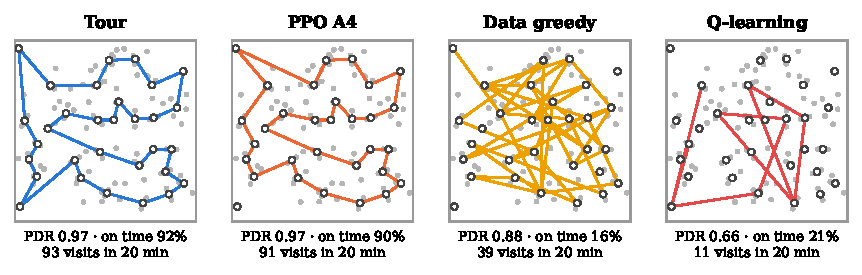
\includegraphics[width=\textwidth]{figures/routes.pdf}
\caption{The same 20 minutes (30--50\,min) of one mission on an unseen 100-sensor network (network
3, stress noise). Grey dots are sensors, circles are meeting points. The tour and PPO fly the same
loop; data greedy and Q-learning cross the field after full buffers, break most of their promises
and make far fewer visits. Numbers below each map are for the whole mission.}
\label{fig:routes}
\end{figure*}

\begin{table}[t]
\caption{Results on ten unseen networks with the stress noise (mean $\pm$ 95\% confidence
interval). On-time: share of promised meetings kept. CH energy: mean energy of a primary
CH.}\label{tab:main}
\centering\small
\setlength{\tabcolsep}{4pt}
\resizebox{\columnwidth}{!}{%
\begin{tabular}{@{}lccc@{}}
\toprule
Policy & PDR & On-time & CH energy (J) \\
\midrule
Tour, fixed window       & $0.972\pm0.006$ & $0.852\pm0.051$ & $96.8\pm12$ \\
Tour, adaptive window    & $0.972\pm0.004$ & $0.910\pm0.022$ & $95.1\pm12$ \\
Nearest feasible         & $0.598\pm0.075$ & $0.867\pm0.019$ & $122\pm13$ \\
Data greedy              & $0.907\pm0.041$ & $0.247\pm0.059$ & $238\pm21$ \\
Energy--data score       & $0.878\pm0.026$ & $0.189\pm0.041$ & $230\pm21$ \\
Q-learning \cite{bouhamed2020uav} & $0.718\pm0.080$ & $0.201\pm0.022$ & $245\pm15$ \\
\midrule
PPO A1                   & $0.972\pm0.006$ & $0.859\pm0.041$ & $92.6\pm9.7$ \\
PPO A2                   & $0.971\pm0.008$ & $0.815\pm0.099$ & $108\pm28$ \\
PPO A3                   & $0.972\pm0.006$ & $0.885\pm0.059$ & $113\pm34$ \\
PPO A4                   & $0.973\pm0.005$ & $0.885\pm0.055$ & $114\pm40$ \\
PPO A4P                  & $0.971\pm0.006$ & $0.903\pm0.025$ & $100\pm16$ \\
\bottomrule
\end{tabular}}
\end{table}

\begin{table}[t]
\caption{PPO minus the tour on the same network (mean $\pm$ 95\% confidence interval; none
excludes zero). A1 and A2 are compared with the fixed-window tour, the others with the adaptive
one.}\label{tab:paired}
\centering\small
\resizebox{\columnwidth}{!}{%
\begin{tabular}{@{}lccc@{}}
\toprule
Variant & PDR (pp) & On-time (pp) & CH energy (J) \\
\midrule
A1  & $+0.00\pm0.03$ & $+0.7\pm2.3$ & $-4.2\pm7.8$ \\
A2  & $-0.09\pm0.26$ & $-3.7\pm6.0$ & $+10.8\pm21.0$ \\
A3  & $-0.04\pm0.30$ & $-2.5\pm4.7$ & $+17.6\pm27.4$ \\
A4  & $+0.02\pm0.23$ & $-2.5\pm4.4$ & $+19.2\pm33.8$ \\
A4P & $-0.14\pm0.24$ & $-0.7\pm0.8$ & $+5.0\pm8.2$ \\
\bottomrule
\end{tabular}}
\end{table}

It can be seen from Table~\ref{tab:main} that every PPO variant delivers more data than every
heuristic, keeps about 3.6 times as many meetings as data greedy, and uses less than half its CH
energy. Data greedy still reaches a PDR of 0.907 while missing three out of four meetings,
because the CHs keep listening in retry and discovery windows after each miss; the cost appears
as 2.5 times the CH energy of the tour. Nearest feasible keeps its meetings but leaves far
clusters unvisited (PDR 0.598). Fig.~\ref{fig:routes} shows why on one network: the tour and PPO
fly the same loop, whereas data greedy crosses the field after the fullest buffer and makes 39
visits in 20 minutes against the tour's 93, and every cluster it passes over misses its window.

The Q-learning baseline reaches a PDR of 0.718 and keeps 20\% of its meetings. Its state
describes only the nearest cluster, so it cannot tell the other candidates apart, and on a new
network it often meets states that it never saw in training, where all its values are equal and
it picks a cluster at random. Each such choice breaks a promise, and the same random choices
make its result change between runs on the same networks (a second run gave 0.677). It is also
trained on fewer decisions than PPO, so it is a weak version of the method rather than a fair
measure of the original paper. It does show why we score every cluster from its own features.

Table~\ref{tab:paired} shows that no PPO variant is significantly different from the tour in
PDR, meetings or CH energy. Among the variants, the adaptive window gives the clearest gain: it
raises the meetings kept from 0.852 to 0.910 for the tour and from 0.815 (A2) to 0.885 (A3) for
PPO. The risk term of A4 adds nothing measurable on top of A3, which is expected, since the
adaptive window already absorbs the UAV's usual lateness. One decision takes 1.5\,ms on a laptop
CPU.

\subsection{What Made Training Work}

\begin{table}[t]
\caption{Effect of each training choice (5 unseen networks, A4P settings). The tour reaches
92.4\% on-time, PDR 0.972 and 91\,J.}\label{tab:fixes}
\centering\small
\setlength{\tabcolsep}{3pt}
\resizebox{\columnwidth}{!}{%
\begin{tabular}{@{}lccc@{}}
\toprule
Setup & On-time & PDR & CH (J) \\
\midrule
PPO from scratch & 59\% & -- & -- \\
First reward (no CH term), any learner & 14--62\% & 0.88--0.91 & 200--300 \\
+ CH energy in reward, start from tour & 82.9\% & 0.952 & 124 \\
+ discount by time & 84.8\% & 0.967 & 120 \\
+ copying step that fades out & 87.0\% & 0.967 & 162 \\
+ early penalty (final) & 90.1\% & 0.969 & 131 \\
\bottomrule
\end{tabular}}
\end{table}

Table~\ref{tab:fixes} shows what each training choice adds. Starting from the tour alone is not
enough, since the agent slowly drifts towards fewer, longer decisions. Discounting by time stops
this drift, and the copying step and the early penalty bring the meetings kept up to 90\%.

\subsection{Larger Networks with Reduced Noise}\label{sec:scale}

\begin{figure}[t]
\centering
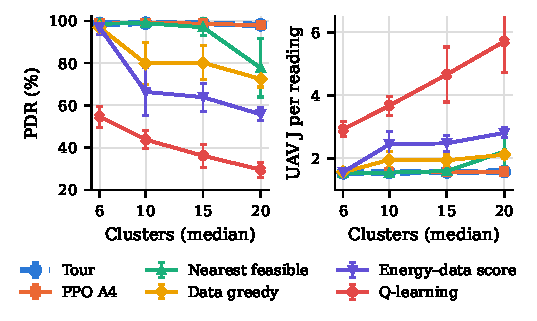
\includegraphics[width=\columnwidth]{figures/ch_sweep.pdf}
\caption{Cluster-count sweep (1000 sensors, reduced noise; mean $\pm$ 95\% CI over ten networks;
x: median number of clusters). Left: PDR. Right: UAV energy per delivered reading. The tour
(dashed) and PPO A4, trained only on 100-sensor networks, lie on top of each other.}
\label{fig:sweep}
\end{figure}

\begin{table}[t]
\caption{PDR on hotspot networks with the reduced noise (mean of ten networks per row; cluster
counts in parentheses are the range over the ten networks). The PPO agent is trained only on
100-sensor networks with even spread.}\label{tab:scale}
\centering\small
\setlength{\tabcolsep}{3pt}
\resizebox{\columnwidth}{!}{%
\begin{tabular}{@{}lcccccc@{}}
\toprule
Networks & Tour & PPO A4 & Nearest & Greedy & En.--data & Q-learn. \\
\midrule
100 sensors, 4 hotspots (4--5)   & 0.994 & 0.994 & 0.993 & 0.992 & 0.991 & 0.983 \\
1000 sensors, 4 hotspots (4--8)  & 0.857 & 0.857 & 0.850 & 0.785 & 0.720 & 0.487 \\
2000 sensors, 4 hotspots (6--8)  & 0.605 & 0.603 & 0.604 & 0.479 & 0.431 & 0.274 \\
\midrule
1000 sensors, target 6 clusters  & 0.987 & 0.987 & 0.987 & 0.970 & 0.969 & 0.547 \\
1000 sensors, target 10 (10--13) & 0.989 & 0.990 & 0.989 & 0.798 & 0.664 & 0.438 \\
1000 sensors, target 15 (13--17) & 0.988 & 0.987 & 0.969 & 0.801 & 0.639 & 0.361 \\
1000 sensors, target 20 (17--24) & 0.981 & 0.979 & 0.777 & 0.725 & 0.558 & 0.296 \\
\bottomrule
\end{tabular}}
\end{table}

For the remaining experiments we use the reduced noise: the UAV speed on each leg is drawn
uniformly from 9--11\,m/s, with no extra delays. We run the same agents, without retraining, on
two sets of networks with sensors packed around hotspots. The first has 4 hotspots with 100,
1000 and 2000 sensors. The second has 1000 sensors with the cluster size capped so that the
networks have about 6, 10, 15 or 20 clusters.

It can be seen from Table~\ref{tab:scale} and Fig.~\ref{fig:sweep} that the agent transfers to networks ten and twenty
times larger than its training networks: A4 stays within 0.2 pp of the tour in every row. The
heuristics fall apart as clusters are added; at 20 clusters, data greedy keeps only 53\% of its
meetings and nearest feasible starts skipping far clusters. Q-learning does not transfer at all
(0.27--0.55 on the 1000- and 2000-sensor networks). The drop at 1000 and 2000 sensors in the
first set is not a routing problem. With only 6--7 clusters, each CH serves 170--290 sensors and
its buffer fills before any UAV can return, so the tour loses 14\% and 39\% of the data to full
buffers, and so does every policy that keeps its promises. The capped networks of the second set
avoid this with more, smaller clusters.

Since the UAV flies or hovers for the whole mission, its total energy hardly differs between
policies (1090--1140\,kJ in the sweep). The energy per delivered reading does: about 1.55\,J for
the tour and PPO at every cluster count, against 2.1--2.8\,J for the heuristics at 15--20
clusters. With the reduced noise the tour keeps every meeting, which confirms that the misses in
Table~\ref{tab:main} come from the extra delays, not from the speed variation.

\subsection{Robustness of the Wake Rule}

\begin{figure}[t]
\centering
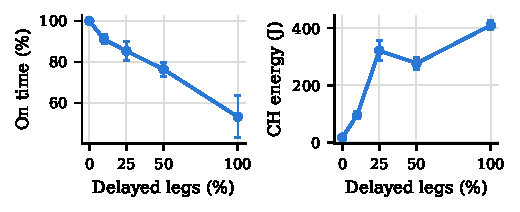
\includegraphics[width=\columnwidth]{figures/uav_delay.pdf}
\caption{Effect of UAV delays on the wake rule (tour, adaptive window, ten 100-sensor networks,
mean $\pm$ 95\% CI). As more legs are delayed by 10--30\,s, fewer meetings are kept and the CHs
spend more energy listening in retry windows; the PDR only falls from 0.973 to 0.932.}
\label{fig:delay}
\end{figure}

\begin{table}[t]
\caption{Robustness of the wake rule (tour with the adaptive window unless stated, ten
100-sensor networks, mean values). Arrows run from the first to the last setting.}\label{tab:robust}
\centering\small
\setlength{\tabcolsep}{3pt}
\resizebox{\columnwidth}{!}{%
\begin{tabular}{@{}llccc@{}}
\toprule
Study & Setting & PDR & On-time & CH energy (J) \\
\midrule
ETA quantile & p80 $\to$ p95 $\to$ p99 & 0.969 $\to$ 0.970 & 76 $\to$ 88 $\to$ 90\% & 321 $\to$ 302 $\to$ 296 \\
UAV delays & 0 $\to$ 50 $\to$ 100\% of legs & 0.973 $\to$ 0.952 $\to$ 0.932 & 100 $\to$ 76 $\to$ 53\% & 17 $\to$ 277 $\to$ 409 \\
CH failures & 0 $\to$ $10^{-4}$ $\to$ $10^{-3}$ per s & 0.973 $\to$ 0.950 $\to$ 0.472 & 91 $\to$ 87 $\to$ 40\% & 98 $\to$ 109 $\to$ 65 \\
CH clock offset & 0 $\to$ 10\,s & 0.972 $\to$ 0.972 & 91 $\to$ 88\% & 95 $\to$ 126 \\
Half-width (no delays) & 5 $\to$ 40\,s & 0.975 $\to$ 0.977 & 99--100\% & 17 \\
\bottomrule
\end{tabular}}
\end{table}

Table~\ref{tab:robust} varies one stress at a time. A wider late side keeps more meetings and
costs less energy, because every missed window is followed by retries: going from the 80th to
the 99th percentile raises the meetings kept from 76\% to 90\% and lowers the CH energy. UAV
delays, not speed noise, are what cause misses (Fig.~\ref{fig:delay}); with every leg delayed, the meetings kept fall to
53\% and the CH energy grows 24-fold, while the PDR drops by only 4 pp. Backup takeover keeps the
PDR at a realistic failure rate, and only at extreme rates do clusters run out of candidates.
Clock offsets of up to 10\,s are absorbed by the window and cost energy rather than data. Without
delays, even a 5\,s half-width keeps every meeting.

\subsection{Can the Tour Be Beaten?}\label{sec:beat}

\begin{table}[t]
\caption{Two cases built to favour leaving the tour (ten unseen 100-sensor networks; burst loss:
share of the data generated during bursts that is lost to full buffers).}\label{tab:bursts}
\centering\small
\setlength{\tabcolsep}{3pt}
\resizebox{\columnwidth}{!}{%
\begin{tabular}{@{}lccc@{}}
\toprule
Policy & PDR & Burst loss & On-time \\
\midrule
\multicolumn{4}{@{}l}{\emph{Small buffers, 20 hotspots (stress noise)}} \\
Tour                                  & 0.896 & -- & 95\% \\
PPO trained on these networks         & 0.896 & -- & 95\% \\
Rule: detour to clusters $\geq$ 70\% full & 0.716 & -- & 53\% \\
Rule: shorter promises at busy clusters & 0.818 & -- & 71\% \\
\midrule
\multicolumn{4}{@{}l}{\emph{Event bursts (reduced noise; PDR $\pm$ 95\% CI)}} \\
Tour                                  & $0.817\pm0.050$ & 0.283 & 100\% \\
Nearest feasible                      & $0.504\pm0.098$ & 0.534 & 93\% \\
Data greedy                           & $0.624\pm0.054$ & 0.528 & 25\% \\
Energy--data score                    & $0.618\pm0.055$ & 0.536 & 19\% \\
Q-learning \cite{bouhamed2020uav}     & $0.451\pm0.052$ & 0.730 & 18\% \\
PPO A4P, trained without bursts       & $0.762\pm0.057$ & 0.366 & 84\% \\
PPO A4P, trained with bursts          & $0.817\pm0.050$ & 0.283 & 100\% \\
\quad same, copying step fades out early & $0.772\pm0.039$ & 0.330 & 81\% \\
\bottomrule
\end{tabular}}
\end{table}

\textbf{Agreement with the tour.} The agent does not simply copy the tour. Right after it is
initialised from the tour, it picks the tour's next cluster at 99\% of decisions, and after PPO
training at 78--87\%. Most of its other choices go first to a cluster whose promise is about to
run out. These changes help on some networks and hurt on others, and they even out.

\textbf{Small buffers.} We first build a case in which the tour loses data: networks with 20
hotspots and CH buffers of 250 readings, where the tour loses 8.9\% of its data to full buffers.
It can be seen from Table~\ref{tab:bursts} that an agent trained on these networks chooses the
tour's next cluster at every decision. Simple rules that follow the tour but detour to any
cluster at least 70\% full do much worse (PDR 0.716, 53\% on-time), since each detour is a long
flight (279\,m per visit against 129\,m on the tour) and every cluster skipped in the meantime
misses its window.

\textbf{Event bursts.} A fixed tour cannot react when one area suddenly produces much more data,
for example during a fire. We therefore add event bursts to the simulator: four times per hour
on average, the sensors of one random cluster read 20 times faster for 30 minutes. A bursting
cluster fills its buffer in about 5 minutes and one tour lap takes about 7 minutes, so the tour
loses 28\% of the burst data. We train A4P on these networks, with its promise choices widened to
$0.5P$--$1.5P$ so that it can promise a quick return to a cluster it finds unusually full. Trained
this way, A4P follows the tour exactly. When the copying step fades out after the first third of
training instead of at the end, the agent leaves the tour more often, but it breaks promises
(81\% on-time) and is 4.5 pp worse than the tour. The heuristics and Q-learning react to full
buffers too, and lose even more. In both cases, therefore, a learned agent either follows the
tour or does worse.

% ---------------------------------------------------------------------------------------------
\section{Discussion}\label{sec:discussion}

\textbf{Why the tour is hard to beat.} Under promise-based wake-up, every CH sleeps until the
time it was promised. Changing the visiting order makes the UAV late somewhere else, and that CH
then misses its window and spends energy on retries. With bursts, the UAV also learns of a burst
only when it next visits that cluster, and going back early breaks promises made to the others.
Leaving the tour therefore costs more than it gains in every case we test, and PPO learning to
match the tour is the expected result, not a training failure.

\textbf{What PPO adds.} The agent was not told that the tour is good; it found it, and it keeps
finding it on networks of 4 to 24 clusters and up to 2000 sensors that it never saw. Every other
policy that plans from the same beliefs, including Q-learning, loses meetings and data as soon as
there are many clusters to choose from. The difference lies in the scoring network, which judges
each cluster from its own features, whereas a single small state cannot tell the candidates
apart.

\textbf{The adaptive window.} The ablation shows that the adaptive window, not the risk term,
gives the clearest gain in meetings kept, for the tour and for PPO alike. Since the window already
absorbs the UAV's usual lateness, a penalty on expected lateness adds little.

\textbf{Scope.} The agents in Tables~\ref{tab:main} and~\ref{tab:scale} are trained only on
100-sensor networks with the stress noise; retraining on the reduced noise and on larger networks
did not finish in time. The Q-learning baseline is our adaptation with a smaller state and less
training, not a reproduction of the original paper. The UAV battery and the return to a depot are
not modelled, and the ablations without backup CHs, with takeover on a missed meeting and without
the start-up lap are implemented but not yet fully evaluated. With ten networks per setting,
differences below about 0.3 pp of PDR are not resolved.

% ---------------------------------------------------------------------------------------------
\section{Conclusions}\label{sec:conclusion}

In this paper, we study how a UAV's visiting order and the wake-up times of the CHs should be
chosen together, and our results are consistent with one account: once every CH sleeps until a
promised time, the shortest tour is already close to the best visiting order. This account ties
together three contributions. First, we propose a promise-then-honour wake rule whose late side
follows the UAV's measured lateness, and we implement the complete system in ns-3; the adaptive
window gives the clearest gain in meetings kept. Second, a PPO agent that scores every cluster
from the UAV's own beliefs matches the shortest tour, beats every heuristic and a tabular
Q-learning baseline, and transfers without retraining from 100 to 2000 sensors and up to 20
clusters. Third, in the cases built to favour leaving the tour, small buffers and sudden traffic
bursts, a learned agent either follows the tour or does worse, because every detour breaks
promises made to other clusters. Together, these results show that under promise-based wake-up
the main value of learning is to keep promises reliably on networks of any size, and that a
policy which beats the tour would need earlier news of a burst, for example from a short status
message of the CH, or a way to change promises already made.

\bibliographystyle{IEEEtran}
\bibliography{refs}

\end{document}
